\subsection{Resultados}
O testes foram feitos com \textit{queries} do tipo leitura e escrita, com duração de 60 segundos, para 1, 5, 10, 15, 20, 30 e 35 clientes em concorrência. Os resultados obtidos correspondem a testes feitos para 1, 2, 3 e 4 réplicas cada uma com 5\% de utilização do cpu.
A métrica analisada corresponde à latência média dos pedidos que foram executados durante um minuto para cada conjunto de clientes em concorrência.

\begin{figure}
    \centering
    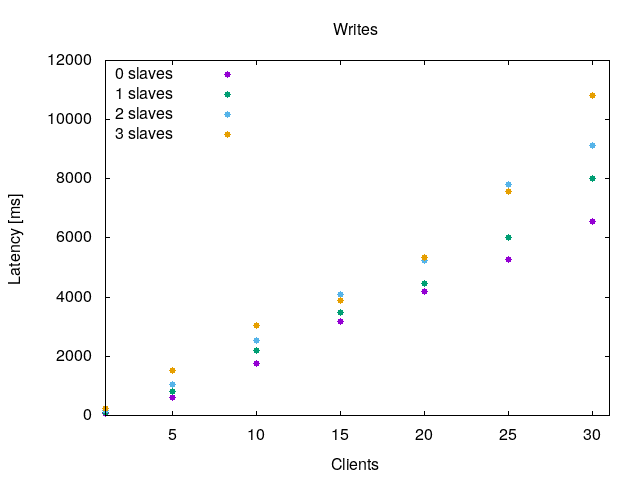
\includegraphics[width=0.9\textwidth]{images/writes.png}
    \caption{Escritas}
    \label{fig:w}
\end{figure}

\begin{figure}
    \centering
    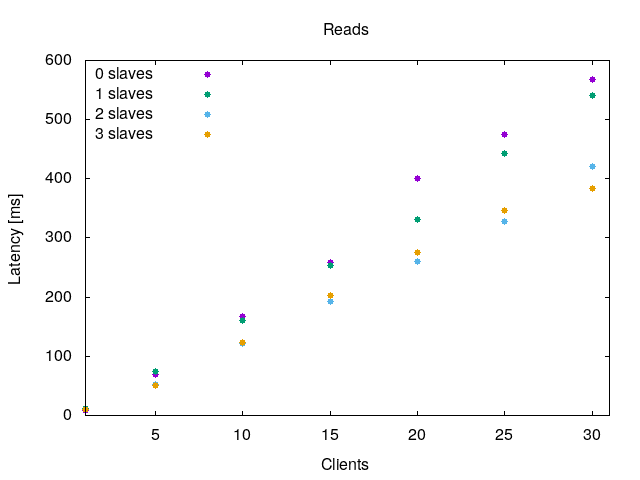
\includegraphics[width=0.9\textwidth]{images/reads.png}
    \caption{Leituras}
    \label{fig:r}
\end{figure}


%Através das tabelas \ref{fig:write_slaves0} a \ref{fig:read_slaves3}, é possível observar o impacto que o PGpool tem nos vários tipos de \textit{queries}. 

Para \textit{queries} de escrita não se verifica melhorias (piora até com o aumento do número de \textit{slaves}), isto porque o PGpool não tem nenhum mecanismo de balanceamento para \textit{queries} deste tipo visto que estas transacções têm sempre de chegar a todos as réplicas.

Já para \textit{queries} de leitura são visíveis as melhorias na latência média dos pedidos, visto que para este tipo de pedidos o PGpool faz balanceamento de carga dividindo os pedidos pelas várias réplicas. 

Num cenário com apenas um cliente a latência média piora quando são utilizados múltiplos \textit{slaves}, isto acontece uma vez que os pedidos estarão a passar pelo PGpool tendo assim um \textit{overhead} adicional. 
Ao comparar os casos de um \textit{cluster} com 3 \textit{slaves} e um com 2 \textit{slaves} (Figura \ref{fig:r}), concluí-se que a latência média só melhora com 30 clientes, verificando que o aumento de réplicas só compensa aumentando também o \textit{workload}.

